% \documentclass[table]{beamer}
\documentclass[table,handout]{beamer}
\setbeameroption{show notes}
% \setbeameroption{hide notes}
% \setbeameroption{show only notes}
\usepackage{varwidth}

\newif\ifhide
\newif\ifpost
\newif\ifhideclicker

% \hidetrue
% \hideclickertrue
% \posttrue

\newcommand{\whiteout}[1]{\textcolor{white}{#1}}
% \newcommand{\whiteoutbox}[1]{\fcolorbox{white}{white}{\parbox{\dimexpr \linewidth-2\fboxsep-2\fboxrule}{\whiteout{#1}}}}
% \newcommand{\notebox}[1]{\fcolorbox{blue}{white}{\parbox{\dimexpr \linewidth-2\fboxsep-2\fboxrule}{#1}}}
\newcommand{\whiteoutbox}[1]{\fcolorbox{white}{white}{\parbox{\linewidth}{\whiteout{#1}}}}
\newcommand{\notebox}[1]{\fcolorbox{blue}{white}{\parbox{\linewidth}{#1}}}
\newcommand{\blankbox}[1]{\phantom{\varwidth{\linewidth}\whiteoutbox{#1}\endvarwidth}}
\newcommand{\blank}[1]{\phantom{\varwidth{\linewidth}#1\endvarwidth}}

\ifhide%
    \newcommand{\hmask}[1]{\blank{#1}}%
\else%
    \newcommand{\hmask}[1]{#1}%
\fi

\ifhide%
    \newcommand{\wout}[1]{\whiteout{#1}}%
\else%
    \newcommand{\wout}[1]{#1}%
\fi

\ifhide%
    \newcommand{\hignore}[1]{}%
\else%
    \newcommand{\hignore}[1]{#1}%
\fi

\ifpost%
    \newcommand{\nopost}[1]{}%
\else%
    \newcommand{\nopost}[1]{#1}%
\fi

\ifhideclicker%
    \newcommand{\clickerslide}[1]{\stepcounter{clickerQuestionCounter}%
        \begin{frame}[t]
            \textcolor{blue}{Q \arabic{clickerQuestionCounter}:}
        \end{frame}}
\else%
    \newcommand{\clickerslide}[1]{#1}%
\fi

\ifhide%
    \newcommand{\hidebox}[1]{\blank{#1}}%
\else%
    \newcommand{\hidebox}[1]{\notebox{#1}}%
\fi

\ifhide%
    \newcommand{\wbox}[1]{\whiteoutbox{#1}}%
\else%
    \newcommand{\wbox}[1]{\notebox{#1}}%
\fi

\ifhide%
    \newcommand{\nbox}[1]{\blankbox{#1}}%
\else%
    \newcommand{\nbox}[1]{\notebox{#1}}%
\fi

\ifhideclicker%
    \newcommand{\clickeranswer}[1]{#1}%
\else%
    \ifhide%
        \newcommand{\clickeranswer}[1]{#1}%
    \else%
        \newcommand{\clickeranswer}[1]{\textbf{\textcolor{blue}{#1}}}%
    \fi
\fi

\usepackage{beamerthemesplit}
% \usetheme{boxes}
\usetheme{Malmoe}
\usecolortheme{seahorse}
% \usecolortheme{seagull}
\usepackage{ifthen}
\usepackage{xspace}
\usepackage{multirow}
\usepackage{multicol}
\usepackage{booktabs}
\usepackage{xcolor}
\usepackage{wasysym}
\usepackage{comment}
\usepackage{hyperref}
\hypersetup{pdfborder={0 0 0}, colorlinks=true, urlcolor=blue, linkcolor=blue, citecolor=blue}
\usepackage{changepage}
\usepackage[compatibility=false]{caption}
\captionsetup[figure]{font=scriptsize, labelformat=empty, textformat=simple, justification=centering, skip=2pt}
\usepackage{tikz}
\usetikzlibrary{trees,calc,backgrounds}

\usepackage[bibstyle=joaks-slides,maxcitenames=3,mincitenames=1,backend=biber]{biblatex}

\newrobustcmd*{\shortfullcite}{\AtNextCite{\renewbibmacro{title}{}\renewbibmacro{in:}{}\renewbibmacro{number}{}}\fullcite}

\newrobustcmd*{\footlessfullcite}{\AtNextCite{\renewbibmacro{title}{}\renewbibmacro{in:}{}}\footfullcite}

% Make all footnotes smaller
% \renewcommand{\footnotesize}{\scriptsize}

\definecolor{myGray}{gray}{0.9}
\colorlet{rowred}{red!30!white}

\setbeamertemplate{blocks}[rounded][shadow=true]

\setbeamercolor{defaultcolor}{bg=structure!30!normal text.bg,fg=black}
\setbeamercolor{block body}{bg=structure!30!normal text.bg,fg=black}
\setbeamercolor{block title}{bg=structure!50!normal text.bg,fg=black}

\newenvironment<>{varblock}[2][\textwidth]{%
  \setlength{\textwidth}{#1}
  \begin{actionenv}#3%
    \def\insertblocktitle{#2}%
    \par%
    \usebeamertemplate{block begin}}
  {\par%
    \usebeamertemplate{block end}%
  \end{actionenv}}

\newenvironment{displaybox}[1][\textwidth]
{
    \centerline\bgroup\hfill
    \begin{beamerboxesrounded}[lower=defaultcolor,shadow=true,width=#1]{}
}
{
    \end{beamerboxesrounded}\hfill\egroup
}

\newenvironment{onlinebox}[1][4cm]
{
    \newbox\mybox
    \newdimen\myboxht
    \setbox\mybox\hbox\bgroup%
        \begin{beamerboxesrounded}[lower=defaultcolor,shadow=true,width=#1]{}
    \centering
}
{
    \end{beamerboxesrounded}\egroup
    \myboxht\ht\mybox
    \raisebox{-0.25\myboxht}{\usebox\mybox}\hspace{2pt}
}

\newenvironment{mydescription}{
    \begin{description}
        \setlength{\leftskip}{-1.5cm}}
    {\end{description}}

\newenvironment{myitemize}{
    \begin{itemize}
        \setlength{\leftskip}{-.3cm}}
    {\end{itemize}}

% footnote without a marker
\newcommand\barefootnote[1]{%
  \begingroup
  \renewcommand\thefootnote{}\footnote{#1}%
  \addtocounter{footnote}{-1}%
  \endgroup
}

% define formatting for footer
\newcommand{\myfootline}{%
    {\it
    \insertshorttitle
    \hspace*{\fill} 
    \insertshortauthor, \insertshortinstitute
    % \ifx\insertsubtitle\@empty\else, \insertshortsubtitle\fi
    \hspace*{\fill}
    \insertframenumber/\inserttotalframenumber}}

% set up footer
\setbeamertemplate{footline}{%
    \usebeamerfont{structure}
    \begin{beamercolorbox}[wd=\paperwidth,ht=2.25ex,dp=1ex]{frametitle}%
        % \Tiny\hspace*{4mm}\myfootline\hspace{4mm}
        \tiny\hspace*{4mm}\myfootline\hspace{4mm}
    \end{beamercolorbox}}

% remove navigation bar
\beamertemplatenavigationsymbolsempty

\makeatletter
    \newenvironment{noheadline}{
        \setbeamertemplate{headline}[default]
        \def\beamer@entrycode{\vspace*{-\headheight}}
    }{}
\makeatother

\newcounter{clickerQuestionCounter}
\ifhideclicker%
\newenvironment{clickerquestion}
{ \stepcounter{clickerQuestionCounter}
  \begin{enumerate}[Q \arabic{clickerQuestionCounter}:]\color{white} }
{ \end{enumerate} }
\else%
\newenvironment{clickerquestion}
{ \stepcounter{clickerQuestionCounter}
  \begin{enumerate}[Q \arabic{clickerQuestionCounter}:] }
{ \end{enumerate} }
\fi

\ifhideclicker%
\newenvironment{clickeroptions}
{ \begin{enumerate}[\begingroup\color{white} 1)\endgroup]\color{white} }
{ \end{enumerate} }
\else%
\newenvironment{clickeroptions}
{ \begin{enumerate}[\begingroup\color{red} 1)\endgroup] }
{ \end{enumerate} }
\fi


\tikzstyle{centered} = [align=center, text centered, font=\sffamily\bfseries]
\tikzstyle{skip} = [centered, inner sep=0pt, fill]
\tikzstyle{empty} = [centered, inner sep=0pt]
\tikzstyle{inode} = [centered, circle, minimum width=4pt, fill=black, inner sep=0pt]
\tikzstyle{tnode} = [centered, circle, inner sep=1pt]
\tikzset{
  % edge styles
  level distance=10mm,
  mate/.style={edge from parent/.style={draw,distance=3pt}},
  mleft/.style={grow=left, level distance=10mm, edge from parent path={(\tikzparentnode.west)--(\tikzchildnode.east)}},
  mright/.style={grow=right, level distance=10mm, edge from parent path={(\tikzparentnode.east)--(\tikzchildnode.west)}},
  % node styles
  male/.style={rectangle,minimum size=4mm,fill=gray!80},
  female/.style={circle,minimum size=4mm,fill=gray!80},
  amale/.style={male,fill=red},
  afemale/.style={female,fill=red},
}

\newcommand{\highlight}[1]{\textcolor{violet}{\textit{\textbf{#1}}}}
\newcommand{\super}[1]{\ensuremath{^{\textrm{\sffamily #1}}}}
\newcommand{\sub}[1]{\ensuremath{_{\textrm{\sffamily #1}}}}
\newcommand{\dC}{\ensuremath{^\circ{\textrm{C}}}}
\newcommand{\tb}{\hspace{2em}}
\providecommand{\e}[1]{\ensuremath{\times 10^{#1}}}
\newcommand{\myHangIndent}{\hangindent=5mm}

\newcommand{\spp}[1]{\textit{#1}}

\newcommand\mybullet{\leavevmode%
\usebeamertemplate{itemize item}\hspace{.5em}}

\makeatletter
\newcommand*{\rom}[1]{\expandafter\@slowromancap\romannumeral #1@}
\makeatother

\newcommand{\blankslide}{{\setbeamercolor{background canvas}{bg=black}
\setbeamercolor{whitetext}{fg=white}
\begin{frame}<handout:0>[plain]
\end{frame}}}

\newcommand{\whiteslide}{
\begin{frame}<handout:0>[plain]
\end{frame}}

\newcommand{\f}[1]{\ensuremath{F_{#1}}}
\newcommand{\x}[1]{X\ensuremath{^{#1}}}
\newcommand{\y}[1]{Y\ensuremath{^{#1}}}

% Population growth macros
\newcommand{\popsize}[1]{\ensuremath{N_{#1}}}
\newcommand{\popgrowthratediscrete}[1]{\ensuremath{\lambda_{#1}}}
\newcommand{\popgrowthrate}[1]{\ensuremath{r_{#1}}}
\newcommand{\ptime}{\ensuremath{t}\xspace}

\tikzset{hide on/.code={\only<#1>{\color{white}}}}
\tikzset{
    invisible/.style={opacity=0},
    visible on/.style={alt={#1{}{invisible}}},
    alt/.code args={<#1>#2#3}{%
        \alt<#1>{\pgfkeysalso{#2}}{\pgfkeysalso{#3}}
        % \pgfkeysalso doesn't change the path
    },
}

\bibliography{../bib/references}
\author[J.\ Oaks]{
    %Jamie R.\ Oaks\inst{1}
    Jamie R.\ Oaks
}
\institute[BIOL 180]{
    \inst{}%
        BIOL 180: Introductory Biology
}



\title{Conservation: Threats \& strategies}
% \date{\today}
\date{June 3, 2015}

% \setbeamertemplate{section in toc}[sections numbered]
% \setbeamertemplate{subsection in toc}[subsections numbered]

\begin{document}

\begin{noheadline}
\maketitle
\end{noheadline}

\nopost{
\begin{noheadline}
\begin{frame}[c]
    \vspace{-6mm}
    \begin{center} 
        \includegraphics[height=1.2\textheight]{../images/seating-chart-2.pdf}
    \end{center}
\end{frame}
\end{noheadline}
}

% \clickerslide{
% \begin{frame}
%     \begin{clickerquestion}
%         \item Which of the following is the clearest example of a positive
%             feedback on global warming?  

%         \begin{clickeroptions}
%             \item \clickeranswer{In Borneo, rainforests are often underlain by
%                     peat. As soils dry, the peat can begin to burn
%                     underground.}
%             \item Glaciers and the Antarctic icecap are melting, contributing
%                 to a rise in sea levels. 
%             \item The oceans are warming, causing seawater to expand,
%                 contributing to a rise in sea levels. 
%             \item Increased CO\sub{2} levels and temperatures are increasing
%                 NPP on land. 
%         \end{clickeroptions}
%     \end{clickerquestion}
% \end{frame}
% }

\clickerslide{
\begin{frame}
    \begin{clickerquestion}
        \item Which of the following is the clearest example of a positive
            feedback on global warming?  

        \begin{clickeroptions}
            \item Germany and China have started major national initiatives to
                encourage solar power. 
            % \item Glaciers and the Antarctic icecap are melting, contributing
            %     to a rise in sea levels. 
            \item The oceans are warming, causing seawater to expand,
                contributing to a rise in sea levels. 
            \item \clickeranswer{Across the arctic, permafrost is melting.
                    Organic matter in these soils is starting to decay.}
            \item Increased CO\sub{2} levels and temperatures are increasing
                NPP on land. 
        \end{clickeroptions}
    \end{clickerquestion}
\end{frame}
}

\begin{noheadline}
\begin{frame}
\frametitle{Today's issues:}
% \vspace{5mm}
% \tableofcontents[subsectionstyle=hide]
\tableofcontents
\end{frame}
\end{noheadline}

\section{Threats to biodiversity}

\subsection{Is a mass extinction currently underway?}

\begin{frame}[t]
    \begin{adjustwidth}{-2em}{-1.5em}
        Is a mass extinction currently underway?

        \uncover<2->{
        \vspace{2mm}
        Data on recent extinctions:
        }

        \begin{enumerate}
            \item<3-> Since year 1000, $\approx$1000 bird species have gone
                extinct; this is 100$\times$ the normal (background) rate.

            \begin{itemize}
                \item NOTE: this is a conservative estimate. 2000 species may
                    have gone extinct in Polynesia alone, due to human
                    colonization.
            \end{itemize}

            \vspace{8mm}
            \item<4-> 122 amphibian species have gone extinct in the past 25
                years.  This is 211$\times$ the background rate.
        \end{enumerate}
    \end{adjustwidth}
    % \note[item]{Tell the David Steadman story}
    \note[item]{Background extinction = extinction rates, due to normal rates
        of environmental change}
    \note[item]{Mass extinction = At least 60\% of species go extinct in less
        than 1 million years; due to extreme rates of environmental change}
    \note[item]{Introduction of mosquitoes and malaria to Hawaii; decimated
        native bird species below 5000ft elevation (E.g., 43 of 65
        honeycreepers extinct)}
\end{frame}

\begin{frame}[t]
    \begin{adjustwidth}{-2em}{-1.5em}
        IUCN data on \% of known species threatened with extinction:

        \uncover<2->{
        \vspace{8mm}
        \begin{table}%[htbp]
            \centering
            \begin{tabular}{ l l }
                Group       & \% \\
                \hline
                Mammals     & 26 \\
                Amphibians  & 41 \\
                Birds       & 13 \\
                Gymnosperms & 40 \\
            \end{tabular}
        \end{table}

        \vspace{4mm}
        NOTE: These are the only groups that are well-studied enough that most
        known species have been evaluated.
        }

    \end{adjustwidth}
    \note[item]{IUCN = International Union for Conservation of Nature; maintain
        Red list of threatened species}
\end{frame}

\begin{frame}[t]
    \begin{adjustwidth}{-2em}{-1.5em}
        IUCN reported 10,553 eukaryotic species were threatened with extinction
        in 1998 (based on objective, quantitative criteria), and 22,413 in
        2014.

        \uncover<2->{
        \[
            \popsize{\ptime} = \popsize{0} \popgrowthratediscrete{}^{\ptime} \,\,\,\,\,\,\,\,\,\,\,\,\,\,\,\,
            \popgrowthratediscrete{} = e^{\popgrowthrate{}} \,\,\,\,\,\,\,\,\,\,\,\,\,\,\,\,
            \popsize{\ptime} = \popsize{0} e^{\popgrowthrate{}\ptime}
        \]
        }

        \vspace{5mm}
        \uncover<3->{
        What is the instantaneous rate of growth of the population of species
        threatened with extinction?

        \nbox{$22413 = 10553 e^{\popgrowthrate{}(16years)} \,\,\, \popgrowthrate{} = 0.047$}
        }
    \end{adjustwidth}
\end{frame}

\clickerslide{
\begin{frame}[t]
        \[
            \popsize{\ptime} = \popsize{0} \popgrowthratediscrete{}^{\ptime} \,\,\,\,\,\,\,\,\,\,\,\,\,\,\,\,
            \popgrowthratediscrete{} = e^{\popgrowthrate{}} \,\,\,\,\,\,\,\,\,\,\,\,\,\,\,\,
            \popsize{\ptime} = \popsize{0} e^{\popgrowthrate{}\ptime}
        \]

        \begin{clickerquestion}
            \item It is estimated that there are 8.7 million species of
                eukaryotes on Earth. Assume the rate of extinction is what we
                just calculated ($\popgrowthrate{} = 0.047$), and 5500
                eukaryotic species have gone extinct due to human activity. How
                long will it take a mass extinction event to occur, starting
                from today?

                \begin{clickeroptions}
                    \item \clickeranswer{146 years}
                    \item 252 years
                    \item 1,018 years
                    \item 8,998 years
                    \item 210,014 years
                \end{clickeroptions}
        \end{clickerquestion}
        \nbox{$8700000\times0.6 = 5500 e^{0.047t}$}

    \note[item]{Mass extinction = 60\% of species go extinct in less than 1
        million years}
\end{frame}
}

\begin{frame}[t]
    \begin{adjustwidth}{-2em}{-1.5em}
        \begin{itemize}
            \item Is the estimate of $\popgrowthrate{}$ that you calculated
                inflated by ascertainment bias?

                \nbox{Yes. IUCN's 2014 estimate of the number of threatened
                    species is based on more data than the 1998 estimate. So,
                    some of the species that were added to the threatened list
                    between 1998 and 2014 were probably already threatened in
                    1998, but IUCN did not know it.}

                \vspace{4mm}
            \item Given projections for human population growth, is the
                estimate for $\popgrowthrate{}$ that you calculated likely to
                be conservative or inflated?

                \nbox{Conservative. 4 billion more people by the end of the
                    century. This will likely greatly exacerbate habitat loss
                    and overexploitation of species}
        \end{itemize}
    \end{adjustwidth}
\end{frame}

\subsection{Why are species going extinct?}

\begin{frame}[t]
    \begin{adjustwidth}{-2em}{-1.5em}
        \vspace{-3mm}
        Data on endangered species from Canada (reflect global trends)

        \vspace{-1mm}
        \begin{center}
            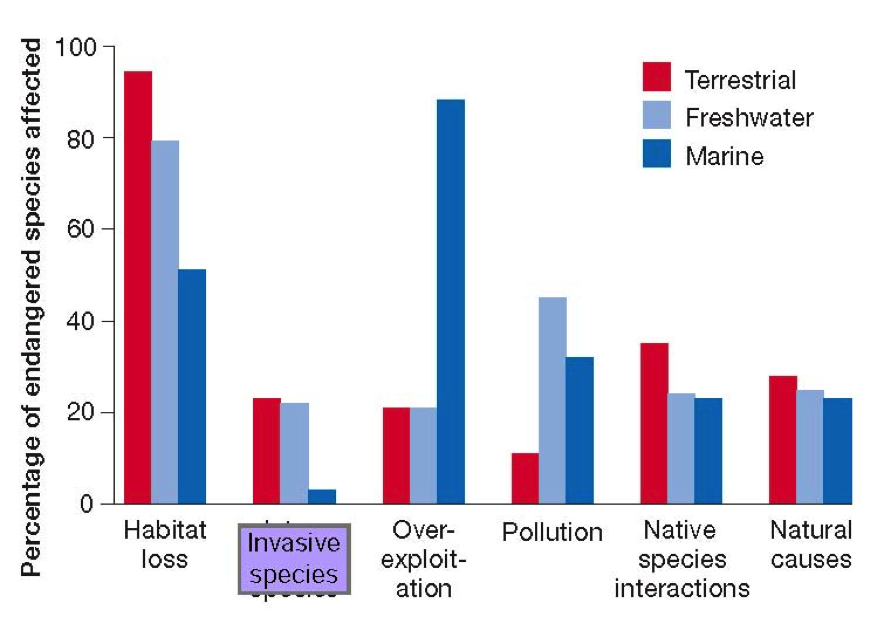
\includegraphics[width=0.7\linewidth]{endangered-threats.png}
        \end{center}

        \vspace{-4mm}
        \begin{itemize}

            \item What is the biggest threat for terrestrial species?

                \nbox{Habitat loss}

            \item What is the biggest threat for marine species?

                \nbox{Overexploitation}
        \end{itemize}
    \end{adjustwidth}
\end{frame}

\clickerslide{
\begin{frame}[t]
    \begin{adjustwidth}{-2em}{-1.5em}
        \vspace{-3mm}
        \begin{center}
            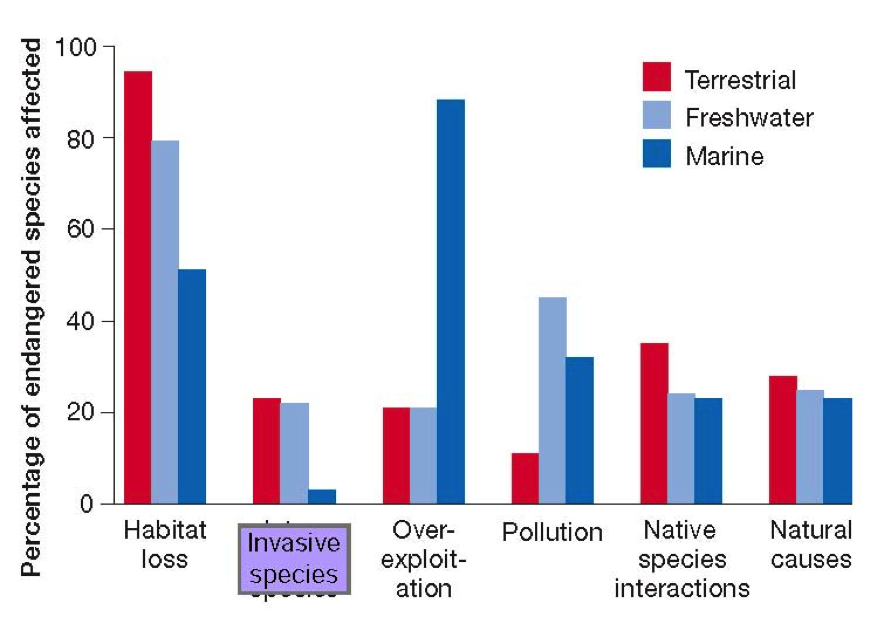
\includegraphics[width=0.55\linewidth]{endangered-threats.png}
        \end{center}

        \begin{clickerquestion}
            \item Why do the percentages for each color add up to more than
                100?
        \end{clickerquestion}

        \begin{clickeroptions}
            \item They represent different types of environments (terrestrial,
                freshwater, marine).
            \item The assessments are subjective.
            \item The assessments are uncertain (need more data).
            \item \clickeranswer{Many species are affected by more than one
                    issue.}
        \end{clickeroptions}
    \end{adjustwidth}
\end{frame}
}

\begin{frame}[t]
    \begin{adjustwidth}{-2em}{-1.5em}
        \vspace{-3mm}
        Data on forest loss (UN FAO):

        \begin{table}%[htbp]
            \centering
            \begin{tabular}{ l c }
                & Global net loss \\
                \cline{2-2}
                1990s & 4.1M ha/yr \\[2ex]
                2000--2005 & 6.4M ha/yr \\
            \end{tabular}
        \end{table}

        \vspace{2mm}
        Total net losses over this interval = 72.9M ha ($\approx$4 WA states)

        \begin{uncoverenv}<2->
        \begin{enumerate}
                \small
            \item What is meant by ``net loss''?

                \nbox{\scriptsize Accounts for re-planting/re-growth}

            \item UN FAO defines ``forest'' as  $\geq$10\% tree cover. Why
                might this be problematic?

                \nbox{\scriptsize Biologists (and other species) would not
                    consider 10\% cover as a functioning forest ecosystem}

            \item The net rate of loss in the tropics is $\approx$70\% higher
                than the global averages above. Why is this concerning?

                \nbox{\scriptsize The tropics contain the most biodiversity,
                    and have the highest NPP}

            \item What is habitat destruction doing to species' distributions?

                \nbox{\scriptsize They are being forced into small,
                    geographically isolated fragments, with limited gene flow
                    (metapopulations with limited migration).}

        \end{enumerate}
        \end{uncoverenv}
    \end{adjustwidth}
    \note[item]{UN FAO = United Nations Food and Agriculture Organization}
\end{frame}

\clickerslide{
\begin{frame}
    \begin{clickerquestion}
        \item Small, isolated populations are more likely than large,
            contiguous populations to go extinct for stochastic (chance)
            reasons that are unrelated to genetics or selection. Why?   
        \begin{clickeroptions}
            \item They do not have alleles that allow them to adapt to changes
                in the environment. 
            \item Mutation rates increase due to small population size and
                physical stress. 
            \item \clickeranswer{They are less likely to survive disturbances.}
            \item They are more likely to suffer from sex ratio or other mating
                problems.
        \end{clickeroptions}
    \end{clickerquestion}
\end{frame}
}

\begin{frame}[t]
    \begin{adjustwidth}{-2em}{-1.5em}
        \vspace{-3mm}
        How do the following processes affect genetic diversity and fitness of
        populations, as they become smaller and more isolated?

        \begin{itemize}
            \item Inbreeding depression
            
                \nbox{\scriptsize In small isolated populations, more
                    deleterious recessive alleles are expressed as homozygosity
                    increases. This lowers the average fitness of the
                    population. Selection will remove such alleles at a higher
                    rate, which will decrease genetic diversity.}

            \item Genetic drift

                \nbox{\scriptsize In small isolated populations, alleles will
                    be lost or fixed at a higher rate do to larger random
                    changes in allele frequencies each generation. Most
                    mutations are deleterious, and more of them will fix due to
                    chance, so the average fitness will decrease.}
        \end{itemize}

        How will changes in the environment affect the fitness of populations
        as they become smaller and more isolated?

        \nbox{\scriptsize As the environment changes, there will be less
            genetic diversity due to the processes above. As genetic diversity
            decreases, the probability that the population will contain alleles
            with high fitness in the new environment decreases. So, the average
            fitness will tend to decrease.}

        How can this lead to an ``extinction vortex''?

        \nbox{\scriptsize As populations become small and isolated, all the
            mechanisms above will lead to decreasing genetic diversity and
            fitness. Thus, the population will likely become even smaller,
            which will increase the intensity of the above mechanisms, which
            will make the population shrink even more, and so on and so on.
            Also, as the population shrinks, random disturbances (fires,
            floods, disease outbreaks, etc.) have a larger affect.}
    \end{adjustwidth}
\end{frame}


\section{How can we reduce threats?}

\subsection{How can we design effective protected areas?}

\begin{frame}[t]
    \begin{adjustwidth}{-2em}{-1.5em}
        \vspace{-3mm}
        How can we design effective protected areas?

        \vspace{2mm}
        Establishing wildlife corridors

        \uncover<2->{
        \begin{itemize}
            \item Experiment with connected vs.\ unconnected patches
                in longleaf pine woodlands (Southeastern USA)
        \end{itemize}

        \begin{center}
            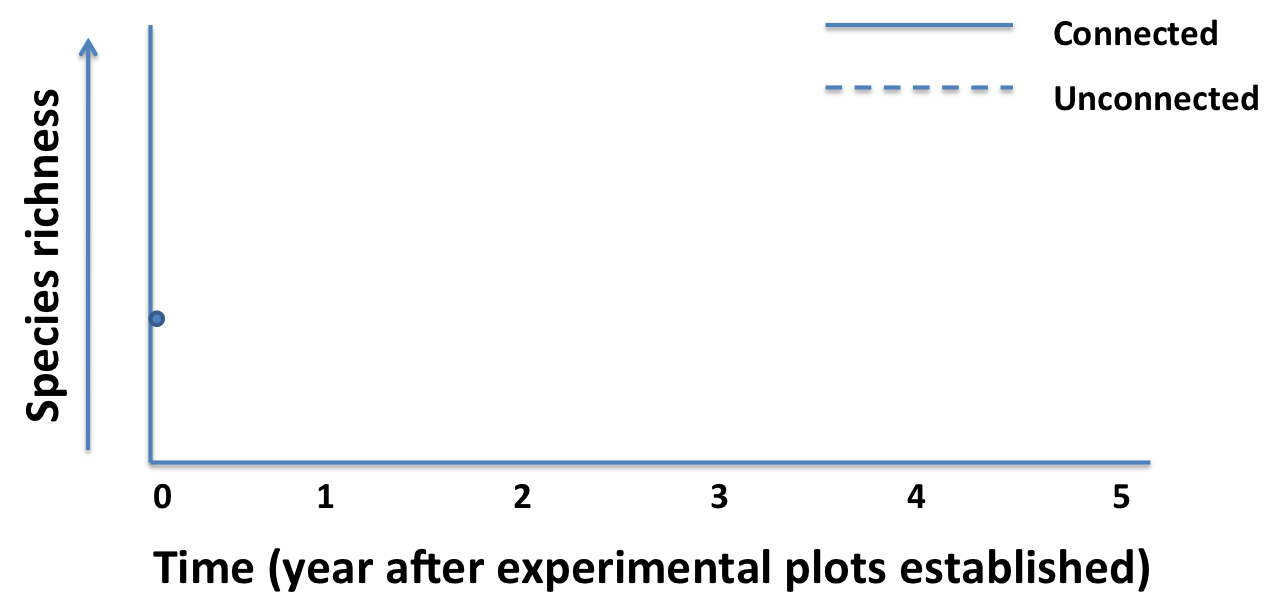
\includegraphics[width=0.85\linewidth]{species-richness-by-time.png}
        \end{center}
        }

        \uncover<3->{
        \vspace{-2mm}
        Why do corridors work?

        \nbox{\tiny Gene flow among small, isolated populations mitigate all
            the issues discussed on the previous slide. Also, allows for
            recolonization if local populations do go extinct.}
        }
    \end{adjustwidth}
\end{frame}

\begin{frame}[t]
    \begin{adjustwidth}{-2em}{-1.5em}
        New issue: How does research on wildlife corridors relate to climate
        change?

        \nbox{Many species will need to move to track their climate niche; they
            will need corridors to do so. Need to predict which regions are
            most likely to support species as climate changes, and plan
            conserving areas and corridors accordingly.}

        Is ``assisted migration'' a good or bad idea? E.g., \spp{Torreya
            taxifolia} from Florida to North Carolina.

        \nbox{Most ecologists think this is a bad idea; potential for
            disrupting existing communities. If done, it needs to be guided by
            LOTS of research to avoid such problems.}
    \end{adjustwidth}
    \note[item]{Famous example of \spp{Torreya} tree going extinct in FL due to
        changing environment. Suitable habitat in NC. People went out at night,
        dug up some of remaining trees and planted them in NC (guerilla
        conservation work).}
\end{frame}

% \subsection{Controlling invasives}

% \begin{frame}[t]
%     Controlling invasives

%     \begin{itemize}
%         \item Purple loosestrife (imported from Europe) was taking over large
%             expanses of marshes in North America

%         \item A researcher found two species of beetle that feed ONLY on
%             purple loosestrife

%         \item Purple loosestrife is now largely controlled in areas where the
%             beetles have been released
%     \end{itemize}
% \end{frame}

% \clickerslide{
% \begin{frame}
%     \begin{clickerquestion}
%         \item Why was it important to confirm that the beetles eat ONLY purple
%             loosestrife? 

%         \begin{clickeroptions}
%             \item To make sure that they will actually eat the target species.  
%             \item \clickeranswer{If they also fed on native vegetation, the
%                     beetles could become an invasive.} 
%             \item Research has shown that primary producers can only be
%                 controlled by specialist consumers. 
%             \item Otherwise, they might not have enough to eat and the
%                 introductions would fail. 
%         \end{clickeroptions}
%     \end{clickerquestion}
% \end{frame}
% }
    

\section{What can we do locally to mitigate threats?}

\subsection{Restoring damaged ecosystems?}

\begin{frame}[t]
    \begin{adjustwidth}{-2em}{-1.5em}
        How can we restore damaged ecosystems?
        
        \begin{itemize}[<+->]
            \item Wangari Maathai---the Green Belt Movement

                \begin{itemize}
                    \item Started in 1977, this NGO has now organized
                        the planting of over 51 million trees in Kenya

                    \nbox{Ms.\ Maathai won the 2004 Nobel Peace Prize. Green
                        Belt Movement has gone international; also focused on
                        women's rights/education/political empowerment}
                \end{itemize}

            \item Local examples of restoration projects:

                \nbox{GreenSeattle restoration along Burke Gilman trail, just
                    north of campus}
                \nbox{UW---native vegetation plantings in the Montlake Fill
                    (Union Bay Natural Area}
                \nbox{Seattle Parks and Rec---Urban Forest Restoration}
                \nbox{GreenSeattle---forest restoration in Magnuson Park}

        \end{itemize}

    \end{adjustwidth}
\end{frame}

\subsection{Lowering our ``ecological footprints?''}

\begin{frame}[t]
    \begin{adjustwidth}{-2em}{-1.5em}
        How can we lower our ``ecological footprints?''

        \vspace{2mm}
        An ``ecological footprint'' is an estimate of how many hectares of
        productive land it takes to support your lifestyle.

        \begin{itemize}
            \item Food:

                % \nbox{Eat at lower trophic levels. Eat local.}
                \vspace{15mm}
            \item Transportation:

                \vspace{15mm}
            \item Goods/services:

        \end{itemize}
    \end{adjustwidth}
    \note[item]{Ask students to talk/think and fill in chart}
\end{frame}


\clickerslide{
\begin{frame}
    \begin{clickerquestion}
        \item Which of the following is the most important part of the
            ``shelter'' footprint, in terms of minimizing it? 

        \begin{clickeroptions}
            \item Location: country and state/province
            \item Design, type of air-conditioning/heating system and building
                materials
            \item \clickeranswer{Number of people per square foot (density)}
            \item How far the home is from work/recreation/shopping
            \item Age of the dwelling
        \end{clickeroptions}
    \end{clickerquestion}
\end{frame}
}


\end{document}

\clickerslide{
\begin{frame}
    \begin{clickerquestion}
        \item 
        \begin{clickeroptions}
            \item 
            \item 
            \item 
            \item 
        \end{clickeroptions}
    \end{clickerquestion}
\end{frame}
}

\clickerpost{
{
\usebackgroundtemplate{\includegraphics[page=17,width=\paperwidth]{./24-Radiation-extinction.pdf}}
\begin{frame}[t,plain]
    \begin{adjustwidth}{-2em}{-1.5em}
        \cmask{Answer: 3}
    \end{adjustwidth}
\end{frame}
}
}

